\chapter{妨碍写作的借口都“貌似有理”}
写作是一项严峻的挑战,就好像修理污水管或是经营一家殡仪馆。虽然我从未给死尸穿过衣服,但是我敢确定,给尸体作防腐处理要比写一篇关于此项活动的文章来得容易。写作很难,这就是为什么我们当中有那么多人写得那样少。如果你在阅读这本书,那么也许你能体味那种屡屡受挫的感受。每次我和教授或是研究生聊起写作这桩事,他们总是提到很多阻碍因素。他们相信,如果不是这样或那样的因素妨碍了他们,他们本来能够写得更多。我把这些借口称为“貌似有理”的借口。乍一看,这些妨碍写作的借口挺像模像样的,但是只要稍加深究,就会发现它们根本站不住脚。本章将列举几个最为常见的妨碍写作的借口,并教大家如何用最简单的方法来克服它们。

\section{借口一}
“我找不到时间写作”,也可以称为“如果我有更多整块的时间,我就能写得更多了”。

这个借口简直是学术界的“尚方宝剑”。我们都这么说;有些屡屡受挫的作者甚至把它高高举起作为人生指南。但是这个假设根本靠不住,就好像有些人相信人类只使用了脑容量的10\%。正如所有的假设一样,这一借口得以存在是因为它让人感到舒服。人们总是想当然地认为周遭的环境总是和自己作对,而如果时间表上有更多大块的空余时间,就可以有更多的时间用来写作,自然就能写得更多了。系里的同仁们对此表示理解,因为他们自己也觉得找不到时间写作。与同事们一起共同经历灰暗的挫折,从某种程度来说有一种奇怪的窃窃的甜蜜感。

为什么这个借口是假的?关键问题就在“找”字上。当人们赞成这个说法时,我的脑海里总是浮现一幅画面,他们的眼睛在时间表上游走,就好像自然科学家在努力寻找一种名叫“写作时间”的生物,这种生物隐藏得太深了,根本寻不到它们的踪迹。你需要“找时间教书”吗?当然不用——你有一张课表,你按部就班,从不迟到。如果你认为写作时间藏匿在你每周计划的某个角落,你就永远不会写得更多。如果你认为非等到整块的时间,比如春假或是暑假,否则就不能写作的话,那么你也不会写得更多。“找时间”对于写作来说是毁灭性的。以后再也不要这么说了。

相反,你不应该“找时间”,而是“安排时间”来写作。高效的写作者都会制订一个时间表并严格遵守。就这么简单。现在,花几分钟想一下你想要的写作时间表。好好想想你的一周安排:是否每周总有那么一些相对空闲的时间?如果你周二和周四有课,那么周一和周三的早上可能是最好的写作时间。如果你觉得下午或是晚上精神更好,那么就安排在晚些时候。每个人根据自己的其他安排,会有不同的黄金“写作时间”。关键在于规律性,而不在于天数或是小时数。你每周是花一天还是五天来写作并不重要——只要你腾出一段有规律的时间来,把它标在你的周计划表上,然后在这段时间坚持写作。开始的时候,你可以每周安排四个小时左右。等看到你所写的文章字数突飞猛进时,你可以再适当延长写作时间。

每次讨论到写作安排时,人们总是问我:那么你的安排呢?(有些人的口气里带着挑衅的意味,仿佛他们希望我耸耸肩,回答道: “怎么说呢,制订计划这种事情,说起来容易做起来难啊。”)我每周一到周五上午八点到十点用来写作。我起床,煮咖啡,然后坐在我的办公桌前。为了避免干扰,我写作前不查邮件,不洗澡,也不换衣服。简言之,我起床,然后写作。开始和结束的时间可能会前后调整,不过我每个工作日大概写两个小时。我不是一个喜欢早起的人,不过早上写作有很多优势,我能够在被处理邮件、学生约谈和与同事会面等事务淹没之前,抓紧宝贵时间写点东西。

大多数人都有一个既浪费时间又毫无成效的坏习惯,被称作“突击写作“ (binge writing) (Kellogg, 1994)。想写,拖延,为拖延感到万分内疚和焦躁,“突击写作者”(binge writer)最终选择某个周六什么也不做,只写东西。这样他们的负疚感得以缓解,整个“突击写作”的周期又开始循环。“突击写作者”花在为没有写作而感到内疚和不安上的时间,要远远超过制订计划的人花在写作上的时间。当你执行计划时,你就没有时间担心没有写作,抱怨找不到时间写作和沉溺于夏天你能够写多少东西的幻想上了。相反,你在固定的时间写作,然后彻底忘了它。我们有很多比写作更值得关注的事情。比如我总是担心我是不是喝了太多的咖啡或者我的狗是不是又到后院那个恶臭的水塘里喝水,但是我从不担心我要找时间写这本书:我知道我会在明天早上八点钟继续。

当“突击写作者”因他们的坏习惯而遭到质疑时,他们常常自我辩护:此乃天性使然,“我不是那种喜欢制订计划并能严格执行的人”。这根本就是废话。人们拿天性来说事儿,是因为他们不想改变(Jellison, 1993)。那些宣称自己不是“计划达人”的人在其他方面却成了计划专家:他们总是在固定的时间教书,在固定的时间上床,在固定的时间看自己喜欢的电视节目等。我就遇到过自称没有能力坚持每天写作的人,却无论刮风下雨都能够坚持在固定时间出门慢跑。千万不要还没有开始就选择放弃——制订计划是高效写作的唯一秘诀。如果你不打算制订计划,那么请你小心合上这本书,把它弄得像新的一样,然后当作礼物送给那些想成为一个好的写作者的朋友。

你必须坚决地捍卫你的写作时间。记住,你要安排时间写作,而不是找时间写作。你自己决定了这段时间是用来写作的。在这段时间内,你不能与同事、学生或是导师见面与约谈;也不能批改作业或者备课;更不能查阅电子邮件、看报纸或是查看天气预报。关掉你的网络和电话,关上门。(我以前会在办公室的门上挂一个“请勿打扰”的牌子,但可恶的是,这块牌子常被人误解为“他关上了门,但是他想让我知道他在办公室,所以我应该敲门而入” 。)

我得提醒你们,其他人未必会理解你对写作时间的忠诚。人们会希望在这段时间和你开个会,他们并非存心捣乱,只是无法理解你为什么没有时间。他们会怨你不知变通,认为你顽固不化,甚至揣测是不是有其他什么不便道明的原因使你不愿见他们。对我来说,最常见的问题是研究生们希望我能够早上九点见他们——这个时间对他们来说最方便,但是不巧,这正好在我的写作时间内。同样的,有时候我也不得不在写作时间里参加一些会议,因为这是唯一一个对所有与会者来说都方便的时间。

怎样应对这些无心打扰到你的人呢?对他们说“不”——这个词也许不能让你远离毒品(南希·里根\footnote{南希·里根,美国总统里根的夫人,曾在美国发起“对毒品说不”运动。——译者注}除外),但能够帮助你捍卫你的写作时间。你有两个很好的理由说“不”。首先,只有“失败的写作者”才会把你的拒绝当作是对他的挑战。我遇到的所有认真的写作者都非常尊重我对写作时间的坚持。他们也许会有一点不高兴,因为我无法在他们希望的时间安排会面,但是他们都会表示理解,因为制订计划是写作的唯一出路(这些人也会在他们的写作时间里拒绝我的会面要求)。为此而恼怒和满腹牢骚的人都不是好的写作者,所以别受他们拖累。其次,人们不会想要占用你的上课时间、你的家庭聚会时间或是你的睡觉时间,却想要占用你的写作时间,因为他们认为你的写作时间无关紧要。作为一个学者,你是职业的写作者,就像你是一名职业的教师一样。把你的写作时间当成你的上课时间,对那些无心打扰的人说“不”,并解释为什么你不能(注意:是“不能”而不是“不愿意”)打破你的写作计划。如果你不喜欢说“不”,那就撒谎。如果你也不喜欢撒谎,那就用你在读研究生的时候学过的理论:归咎于一个“常见又固定的职责”或是一个“世俗的拖累”。

在既定的写作时间里奋笔疾书,但是也不要教条化地圃于写作时间。如果你在写作时间结束后仍然文思泉涌或者在其他时间里坚持写作,岂不是更好?我把这称为“意外之作”。一旦你养成了习惯,坐下来写东西就会变得容易了。不过你要提高警惕,不能用“意外写作”来替代正常的写作时间。不管你在放春假的时候写了多少——你都应该遵守你的写作计划,严格执行。如果你发现自己胡说——“我周末已经写得够多了,周一我就轻松一下吧”,那这本书能够帮到你:合上它,用你非惯用的那只手的拇指和食指夹住它,在自己面前狂甩五分钟,以便提醒你怎样才是正确的做法。

或许你对“计划写作”是否有效还有保留意见。“这真的就是秘诀吗?”你也许会问,“难道就没有其他的法子能够多写点?”没有了——做好计划并严格执行是唯一的办法。职业写作者拉夫·凯斯(Ralph Keyes,2003: 49)在对成功写作者们的写作习惯做了大量研究后发现,“使一位写作者得以高产的秘诀就是坐在书桌前日复一日地写作”。如果你每周安排四个小时写作,你会对你能够完成的字数感到惊讶,确切地说是震惊,惊得哑口无言,呆若木鸡。你会发现自已完成了之前无法想象的事,例如提早完成了开题报告。你会收到改稿通知,并在一周内完成。你不敢再和系里的同事交流对写作的恐惧,因为你害怕他们会说“你已经不再是我们的战友了”,而且他们的话千真万确。


\section{借口二}
“我需要先作一些数据分析”,或者“我要先看几篇文章”。

这个借口最为阴险,危害也最大。首先,这个借口看起来合情合理。你也许会说,“我总不能既不看参考文献又不作数据分析,就直接写文章吧”。没错,但是我见过很多人把这个借口当作颂歌每日吟唱。同事们一开始都很尊重他们,相信他们要么是完美主义者,要么就是数据狂人。但是他们写得不多,也从不作所谓的数据分析。“突击写作者”往往也是“突击阅读者”和“突击数据分析员”,阻碍他们写作的坏习惯同样会妨碍他们做其他与写作相关的准备工作(Kellogg, 1994)——阅读、列提纲、提炼观点、分析数据,等等。像其他所有“貌似有理”的借口一样,这个借口也经不起深究。

要破解它很容易:在你安排的写作时间内,做一切你需要做的事情。要做一些数据分析吗?在你的计划时间里做。要看一些参考文献吗?在你的计划时间里做。要校验清样吗?也在你的计划时间里完成。要读一本如何写作的书呢?你知道应该什么时候读。写作的含义远不只是坐在电脑前打字,任何与完成写作任务相关的活动均可称为写作。例如,为了完成一篇论文,我常常会连续花几段写作时间来作数据分析。有时候我会花上一整段写作时间来做一些鸡毛蒜皮的事,比如研究某一杂志的投稿要求、画图表或校样稿。

这也是为什么只有制订计划才能够保障写得更多的又一原因。专业的写作包含很多部分:广泛的文献阅读、仔细的分析、文字严谨的研究方法陈述。我们无法“找时间”来完成所有相关文献的检索与阅读,就如同我们无法“找时间”写下阅读这些文章的笔记。所以安排好你的写作时间来完成这些工作吧。这样你就不会为找不到时间来读文献和作分析而感到惶恐了,因为你知道什么时候你会完成它们。


\section{借口三}
“我需要一台新电脑才能更好地写作”(同理,这里的“电脑”可以替换为“新的激光打印机”“新椅子”“新书桌")。

在所有的借口中,这条是最让人抓狂的。我不确定人们是否真的相信它——与其他的借口不同,这一条其实真的只能勉强算是一个“借口”。我自己的实例可能就能破解这个借口。当我还在读研究生时,我刚开始严肃地写作,我从一个同学的男朋友那里买了一台很旧的电脑。这台电脑即使在1996年也可以算是一件古董:没有鼠标,没有Windows,只有一个键盘和DOS系统下的WordPerfect 5.0软件。这台电脑寿终正寝以后,我的一些文件也因为无法复制而随之陪葬了。我又买了一台手提电脑,常常席地埋头苦写。我现在正在用2001年购买的一台速度奇慢、老得掉牙的东芝笔记本电脑写这本书——在如今电脑更新换代如此迅速的时代,我的这台笔记本电脑老得都可以去领养老金了。

大概有八年的时间,我都坐在一把折叠椅上辛勤笔耕。这把折叠椅退休以后,替代它的是一把稍微时髦,但是同样坚硬的老式埃姆斯椅。它是一把再简单不过的椅子:没有装饰和靠垫,也不能调节高度和角度。为了满足大家的好奇心,附上一张我写这本书的地方的图片。如图2.1,只有一张大而简单的书桌(没有抽屉,没有键盘架,没有豪华的文件收纳体系,等等)、一台激光打印机和一个咖啡杯垫。在我买下这张“蓝点”(注:著名家具品牌)书桌以前,我用的是一张10美元的胶合板折叠书桌,为了显示我的品位,上面铺了一块4美元的桌布。我就坐在那把折叠椅上,在那张折叠书桌旁,写完了我那本关于兴趣的专著的大部分内容(Silvia, 2006)和近20篇学术论文。

\begin{figure}[!htb]
\label{fig2-1}
\centering
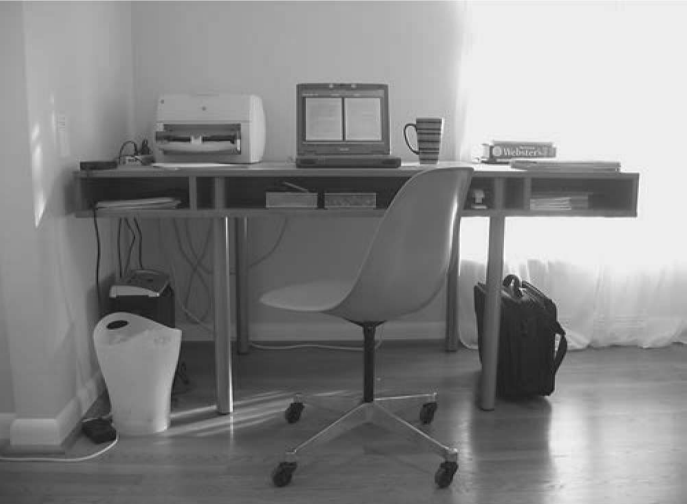
\includegraphics[width=0.9\textwidth]{fig2-1.png}
\caption{我写作本书的地方}
\end{figure}


低效的写作者总喜欢悲悲切切地抱怨没有属于自己的哪怕一小块空间用来写作。我对这个老掉牙的借口不屑一顾。我从来没有专属的家庭办公室或是私人写作空间。在狭小的公寓或是房子里,我在客厅、卧室、客卧、主卧甚至浴室里写作,我只需要一张小桌子。我在家里的客卧里完成了这本书的写作。即使现在,我已经写了那么多书和论文,也买了自己的房子,我在家还是没有独立的书房来写作。我也不需要——总有一间浴室是空着的。

我身边的突击写作者曾多次提到打印机问题是阻碍他们写作的原因之一,他们提到这一问题的频率之高让我颇为吃惊。 “如果我家里有一台激光打印机的话……”他们用充满渴望的口气这样抱怨。他们没有意识到自己不能像印钞票一样打印写作稿——打印机只能用来打印你已经写好的稿子。我非常喜爱我的激光打印机,每个认真的写作者都应该买一台,不过打印机真的不是必需的。当雪莱·杜瓦尔(T. Shelley Duval)和我在合写一本关于自我意识的著作时(Duval \& Silvia, 2001),我只有一台石器时代的喷墨打印机,他什么都没有。要用喷墨打印机打印一本书需要很长的时间,到头来我们的部分草稿还是青绿色和红褐色的,因为打印机的黑墨水用完了。

当人们抱怨他们家里没有高速互联网时,我真心祝贺他们有这样正确的判断。如果你们仔细看图2.1,就会发现我的电脑上根本没接网线。我太太在家里的书房里安装了高速网络,我没有。这玩意儿只会让我分散注意力。写作时间就是用来写作的,不是用来查邮件、看新闻,或是浏览最新期刊的。有时候我会觉得下载一些文章可能对写作有点帮助,不过我可以在办公室里下载。最好的自控就是让客观环境不需要自控。

威廉·萨拉扬(William Saroyan, 1952: 42)这样写道,“写作,你只需要一张纸和一支笔。”设备永远不能帮你写作;只有制订写作计划并努力执行才能帮助你成为一名高效的写作者。如果你不相信我所说的,那么就看看比尔·斯顿夫(Bill Stumpf)最新的采访。作为家具设计业的传奇人物,斯顿夫为业界领军者赫尔曼·米勒(Herman Miller)公司设计办公家具。斯顿夫因为参与了艾龙椅(Acron)的设计而闻名,这真的是有史以来最棒的办公椅了。但是作为一名写作者(Stumpf, 2000),他深知家具能做的只有这些了。 “我不确定家具和写作能力这两者之间是否存在必然联系,”他说,“我想赫尔曼·米勒一定不喜欢听到我这样说
(Grawe, 2005: 77) 。”


\section{借口四}
“我只是在等待对的时机”,或者“我在灵感来临的时候才能写出好的文章”。

这最后一个借口是最可笑和最无厘头的。我无数次从那些不知何故拒绝制订写作计划的人那里听到这样的理由。 “好的作品都是在我有灵感的时候一气呵成的,”他们说,“在我没有心情的时候逼着我写也无济于事。我必须感到我想写了才行。”毫无建树的写作者这样说真是可笑。这就好像烟鬼们总是辩解吸烟能够使他们感到放松,而实际上吸入尼古丁压根儿就只会导致精神紧张(Parrott, 1999)。当那些备受折磨的人为不制订计划而辩解时,他们是在支持使他们深受折磨的原因本身。如果你相信你应该只在有灵感的时候写文章,那就请你问自己几个简单的问题:这种策略效果如何?你对自己文章的数量感到满意吗?你是否常常为找时间写作或是为仅仅完成了一半的论文而感到紧张?你是否牺牲了晚上或是周末的时间用来写作?

要驳倒这个借口也不难:研究表明等待灵感是徒劳的。博伊斯(Boice, 1990: 79$\sim$ 81)为那些等待灵感的突击写作者做了一个意义深远的研究。他召集了一批为写作而头痛的大学教授,随机地给他们分配了不同的写作策略。第一组(限制写作组)的教授们被禁止在任何非紧急情况下写作;第二组(顺其自然组)的教授们有50段写作时间,但是仅在他们感到有灵感的时候写;第三组(附加干预组)的教授们有50段写作时间,并且在这些时间内必须写作(如果他们没写,就得向一个他们不喜欢的组织交罚款)。统计项是每天写作的数量和每天提出的创造性观点的数量。图2.2的数据显示了博伊斯的结论。首先,附加干预组的产量最高:他们的产量是顺其自然组的3.5倍,是限制写作组的16倍。那些只在有灵感的时候写作的人比那些被告知没事别写的人多写了一点点——灵感的作用实在是被高估了。其次,那些被逼着写作的人提出了更多创造性的想法,他们平均提出想法的间隔是1天;顺其自然组是2天,而限制写作组是5天。由此可见,写作本身孕育了继续写下去的基础。

\begin{figure}[!htb]
\label{fig2-2}
\centering
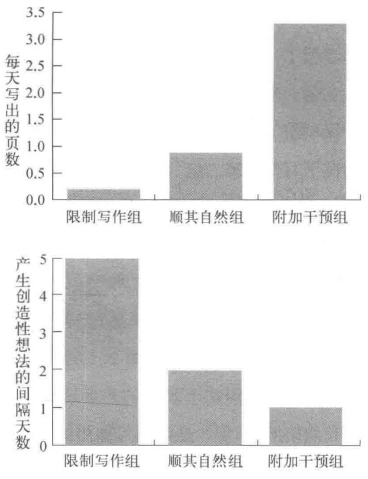
\includegraphics[width=0.9\textwidth]{fig2-2.png}
\caption{不同写作策略的效果}
\end{figure}

有些类型的写作实在太不可爱了,以至于没有一个正常人会喜爱它们。什么样的人会对写开题报告感到热情高涨呢?谁会早上醒来,就对写作“具体目标”和“协议/合约安排”感到欢欣鼓舞呢?写课题申请报告就好像报税,而且你还没法请个会计来帮你做。如果你对阅读美国卫生与公共服务部提供的科研基金SF424申请指南有着难以抑制的热情,那么你根本不需要这本书。如果你和其他人一样,那么要完成课题申请报告,你需要的不仅仅是“灵感”。

那些等待灵感的人应该从云端降落,回归到正常的普通大众当中。古希腊人为诗歌、音乐和悲剧都各分配了一个神,但是从未听说他们为按照美国心理学会(APA)格式写作期刊论文安排了什么神灵。作为学者,我们不是在进行文学创作,也没有书迷等在酒店门口,手捧《人格与社会心理学公报》,要求我们在上面签名。我们写的是专业性的、学术性的文章。有些类型的学术写作可能稍微轻松——例如教科书,或是比如这本书——但是即使这样,也要求我们把有用的信息归纳齐整,然后传递给读者。我们的写作很重要,因为它是实用的、清晰的和启发思考的。

拉夫·凯斯(Ralph Keyes, 2003)告诉我们,最杰出的小说家和诗人——在我们看来最应该等待灵感的人——实际上也并非只在有灵感的时候才写作。高产的安东尼·特罗洛普(Anthony Trollope, 1883$\sim$ 1999:121)这样写道:

\begin{lstlisting}
有些人认为他们为灵感而生,所以他们应该允许自己等待灵感来唤醒他们。每当我听到这样的布道时,总是很难掩饰我内心的不屑。在我看来,没有什么比这种说法更荒诞了,就是一个鞋匠说他要等待灵感,或是牛油烛小商贩在等待神的旨意来融化牛油也没有这么荒诞。有一次有人告诉我最可靠的有助写作的方法是在椅子上涂一点鞋线蜡。我宁愿相信鞋线蜡也不相信灵感。
\end{lstlisting}

那么这些杰出的写作者都怎样写作呢?猜猜看。成功的专业写作者,无论他们写的是小说、非小说、诗歌还是戏剧,他们的高产都有赖于有规律地写作(通常是坚持每天写作)。他们都不相信必须等有了感觉才能写作。正如凯斯(Keyes, 2003: 49) 所说,“认真的写作者笔耕不辍,不论有无灵感。随着时间推移,他们发现规律性显然是比灵感更靠谱的朋友”。有人或许会说,那就订个计划并且严格执行吧。

\section{小结}
本章对一些常见的妨碍写作的借口进行了冷静而批判性的审视。我们都喜欢躲在这些温暖的外衣下,但是披着这温暖的外衣还想码字实在是太难了。如果你还对这些借口恋恋不舍,那就把这章多读几遍,直到你被彻底洗脑而坚信只有制订计划才有未来。如果你不相信这一点,那么这本书恐怕就帮不了你了,因为无论你喜不喜欢写作,能够写得更多的秘诀只有保持规律性地写作。制订好了写作计划,你就可以继续读下一章了。它将介绍一些简单而有效的激励工具,让你能够坚持写作并且提高你的写作效率。